\section{Back-End Server}
The Back-End server instantiates different versions of itself based on command line arguments.
Each instance of a Back-End server is be responsible for listening for a specific type of data:
APRS data, telemetry data or video data. The Back-End server is implemented in Python 2.7 and
uses the socketio and eventlet libraries to communicate events to the Front-End server.
The ArgumentParser and ConfigParser modules are used to support command line arguments and server
configuration.

\begin{figure}[!ht]
  \centering
  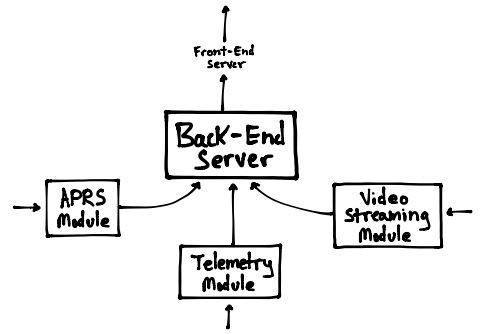
\includegraphics[scale=.8]{imgs/back-end-server.jpg}
  \caption{Back-End Server}
\end{figure}

\subsection{APRS Module}
The APRS module catches raw APRS packets sent by the Recovery Crews and sending on to the Front-End server.
This module relies on the aprslib library to correctly parse incoming APRS packets. It also relies on the 
json library to prepare the parsed APRS packets that are emitted as events by the Back-End server.


\begin{figure}[!ht]
  \centering
  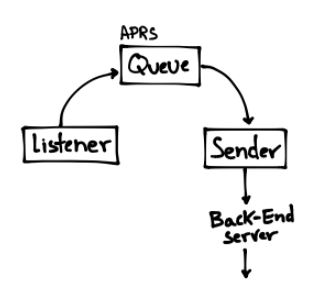
\includegraphics[scale=.8]{imgs/aprs-detailed.jpg}
  \caption{APRS module}
\end{figure}

\newpage

\subsection{Telemetry Module}
The Telemetry module catches raw telemetry data from the rocket and sends it to the Front-End server.
It uses the psas_packet and socket libraries for receiving telemetry data and the Queue library for 
creating a data structure that the listening thread and the broadcasting thread can both access.

\begin{figure}[!ht]
  \centering
  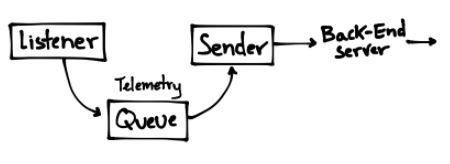
\includegraphics[scale=.8]{imgs/telemetry-detailed.jpg}
  \caption{Telemetry Module}
\end{figure}

\subsection{Video Streaming Module}
The video module catches the live video streams and sending them to the Front-End server.

\begin{figure}[!ht]
  \centering
  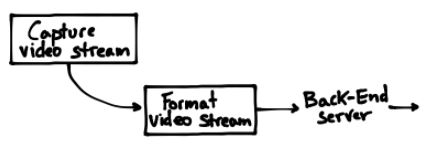
\includegraphics[scale=.8]{imgs/video-detailed.jpg}
  \caption{Telemetry Module}
\end{figure}
